
\documentclass{beamer}
\usecolortheme{dove}
\setbeamertemplate{navigation symbols}{}
\usepackage{amsmath,amssymb,amsfonts,amsthm, multicol, subfigure, color}
\usepackage{bm}
\usepackage{graphicx}
\usepackage{tabularx}
\usepackage{booktabs}
\usepackage{hyperref}
\usepackage{pdfpages}
\usepackage{xcolor}
\definecolor{seagreen}{RGB}{46, 139, 87}
\def\independenT#1#2{\mathrel{\rlap{$#1#2$}\mkern2mu{#1#2}}}
\newcommand\indep{\protect\mathpalette{\protect\independenT}{\perp}}
\def\log{\text{log}}
\newcommand\logit{\text{logit}}
\newcommand\iid{\stackrel{\text{iid}}{\sim}}
\newcommand\E{\text{E}}
\newcommand\V{\text{V}}
\renewcommand\P{\text{P}}
\newcommand{\Cov}{\text{Cov}}
\newcommand{\Cor}{\text{Cor}}
\newcommand\doop{\texttt{do}}
\usepackage{stackrel}
\usepackage{tikz}
\usetikzlibrary{arrows,shapes.arrows,positioning,shapes,patterns,calc}
\newcommand\slideref[1]{\vskip .1cm \tiny \textcolor{gray}{{#1}}}
\newcommand\red[1]{\color{red}#1}
\newcommand\blue[1]{\color{blue}#1}
\newcommand\gray[1]{\color{gray}#1}
\newcommand\seagreen[1]{\color{seagreen}#1}
\newcommand\purple[1]{\color{purple}#1}
\newcommand\orange[1]{\color{orange}#1}
\newcommand\black[1]{\color{black}#1}
\newcommand\white[1]{\color{white}#1}
\newcommand\teal[1]{\color{teal}#1}
\newcommand\magenta[1]{\color{magenta}#1}
\newcommand\Fuchsia[1]{\color{Fuchsia}#1}
\newcommand\BlueGreen[1]{\color{BlueGreen}#1}
\newcommand\bblue[1]{\textcolor{blue}{\textbf{#1}}}
\newcommand\bred[1]{\textcolor{red}{\textbf{#1}}}
\newcommand\bgray[1]{\textcolor{gray}{\textbf{#1}}}
\newcommand\bgreen[1]{\textcolor{seagreen}{\textbf{#1}}}
\newcommand\bref[2]{\href{#1}{\color{blue}{#2}}}
\colorlet{lightgray}{gray!40}
\pgfdeclarelayer{bg}    % declare background layer for tikz
\pgfsetlayers{bg,main} % order layers for tikz
\newcommand\mycite[1]{\begin{scriptsize}\textcolor{darkgray}{(#1)}\end{scriptsize}}
\newcommand{\tcframe}{\frame{
%\small{
\only<1|handout:0>{\tableofcontents}
\only<2|handout:1>{\tableofcontents[currentsubsection]}}
%}
}

\usepackage[round]{natbib}
\bibliographystyle{humannat-mod}
\setbeamertemplate{enumerate items}[default]
\usepackage{mathtools}
\usepackage{ulem}

% Need to add examples

\newcommand{\goalsframe}{\begin{frame}{Learning goals for today}
At the end of class, you will be able to:
\begin{enumerate}
\item Finish the \bref{https://github.com/ilundberg/teaching/blob/master/info_6751_causal/class_exercises/principal_stratification/Info_6751_Principal_Strata_Exercise.pdf}{class exercise} we started on Tuesday [\bref{https://github.com/ilundberg/teaching/blob/master/info_6751_causal/class_exercises/principal_stratification/Info_6751_Principal_Strata_Exercise_Solutions.pdf}{solutions}]
\item See principal stratification in action:\\quantifying racial bias in policing
\end{enumerate} \vskip .2in
\end{frame}}

\title{21. Principal Stratification (Part 2)}
\author{Ian Lundberg\\Cornell Info 6751: Causal Inference in Observational Settings\\Fall 2022}
\date{3 Nov 2022}

\begin{document}

\maketitle

\goalsframe

\begin{frame}{Wrapping up the class exercise: Question 6}{Size of the stratum who have a child regardless of college} \pause
Among those who finish college ($A = 1$),\\
having a child ($M = 1$) is the same as\\
being in the always-child stratum ($S = 1$) \vskip .1in \pause
$$\begin{aligned}
\P(M = 1 \mid A = 1) = \P(S = 1 \mid A = 1)
\end{aligned}$$ \pause
We are assuming $A$ is randomly assigned, so
$$\P(S = 1\mid A = 1) = \P(S = 1)$$ \pause
So $\P(S = 1)$ equals the motherhood rate\\among college women: 0.71
\end{frame}

\begin{frame}{Wrapping up the class exercise: Question 7}{Size of the stratum who have a child only if no college} \pause
Among those who do not finish college ($A = 0$),\\
having a child ($M = 1$) is equivalent to being in either\\
the always-child stratum ($S = 1$) or\\
the child-if-no-college stratum ($S = 3$)\\
 \vskip .1in
$$\begin{aligned}
\P(M = 1 \mid A = 0) = \P(S \in \{1,3\} \mid A = 1)
\end{aligned}$$ \pause
We are assuming $A$ is randomly assigned, so
$$\P(S = \in \{1,3\}\mid A = 0) = \P(S = \in \{1,3\})$$ \pause
So $\P(S \in \{1,3\})$ equals the motherhood rate\\among non-college women: 0.83 \vskip .1in \pause
Estimate $\P(S = 3) = \P(S\in \{1,3\}) - \P(S = 1) = .83 - .71 = .12$
\end{frame}

\begin{frame}{Wrapping up the class exercise: Question 8}{Child outcome under mother college, in the always-child stratum} \pause

$$\begin{aligned}
\mu^1_1 &= \E(Y^1\mid S = 1) \\ \pause
&= \E(Y\mid A = 1, S = 1) &\text{exchangeability} \\ \pause
&= \E(Y\mid A =1) &\text{monotonicity} \\ \pause
&= 0.40
\end{aligned}$$

\end{frame}

\begin{frame}{Wrapping up the class exercise: Question 9}{Child outcome under mother no college, in the always-child stratum} \pause
To identify $\mu^0_1$, first write a formula for $\bar{y}^0$: the mean outcome among non-college women. \vskip .2in \pause
That is a weighted average of outcomes among strata 1 and 3.
$$\begin{aligned}\overbrace{\frac{\pi_1}{\pi_1 + \pi_3}}^{\substack{\text{Proportion}\\\text{in $S = 1$}}}\mu^0_1 + \overbrace{\frac{\pi_3}{\pi_1 + \pi_3}}^{\substack{\text{Proportion}\\\text{in $S = 3$}}}\mu^0_3 &= \overbrace{\bar{y}^0}^{\substack{\text{Mean outcome among}\\\text{non-college mothers}}} \\ \pause
\\
\text{Rearrange to solve for }\mu^0_1&\\ \pause
\frac{\pi_1}{\pi_1 + \pi_3}\mu^0_1 &= \bar{y}^0 - \frac{\pi_3}{\pi_1 + \pi_3}\mu^0_3 \\ \pause
\mu^0_1 &= \frac{\pi_1 + \pi_3}{\pi_1}\left(\bar{y}^0 - \frac{\pi_3}{\pi_1 + \pi_3}\mu^0_3\right)
\end{aligned}$$
\end{frame}

\begin{frame}{Wrapping up the class exercise: Question 10}{Child outcome under mother no college, in the always-child stratum}
$$\mu^0_1 = \frac{\pi_1 + \pi_3}{\pi_1}\left(\bar{y}^0 - \frac{\pi_3}{\pi_1 + \pi_3}\textcolor{blue}{\mu^0_3}\right)$$ \pause
The only unknown term is $\blue{\mu^0_3}$. We can bound it. \pause
$$\begin{aligned}
\hat\mu^{0,\text{Upper}}_1 &= \frac{.71 + .12}{.71}\left(.18 - \frac{.12}{.71 + .12}\textcolor{blue}{\mathbf{1}}\right) = .04  \\ \pause
\hat\mu^{0,\text{Lower}}_1 &= \frac{.71 + .12}{.71}\left(.18 - \frac{.12}{.71 + .12}\textcolor{blue}{\mathbf{0}}\right) = .21
\end{aligned}$$

\end{frame}

\begin{frame}{Wrapping up the class exercise: Question 10}{Set identification for the causal effect} \pause
The causal effect estimate is set-identified by
$$
\begin{aligned}
\hat\tau_1^\text{Lower} &= \hat\mu^1_1 - \hat\mu^{0,\text{Upper}}_1 &= .40 - .21 &= .19 \\
\hat\tau_1^\text{Upper} &= \hat\mu^1_1 - \hat\mu^{0,\text{Lower}}_1 &= .40 - .04 &= .36
\end{aligned}
$$ \vskip .2in \pause

Among women who would have a child\hfill \textcolor{gray}{stratum-}\\regardless of their own education,\hfill\textcolor{gray}{specific}\vskip .1in \pause
the effect of a mother finishing college \hfill\textcolor{gray}{causal} \\
on the probability that her child finishes college \hfill\textcolor{gray}{effect} \vskip .1in \pause 
is somewhere between 0.19 and 0.36.\footnote{(This is of course subject to the doubtful assumptions made in the problem, but even under those strong assumptions the interval is very wide.)}\hfill\textcolor{gray}{set-identified}

\end{frame}

\begin{frame}
Big picture ideas in this exercise \vskip .1in \pause
\begin{itemize}
\item Principal stratification solved a hard problem
\begin{itemize}
\item A mediator that can render an outcome undefined \pause
\end{itemize}
\item You can bound estimates by assuming monotonicity\\(and applying lots of algebra)
\end{itemize}
\end{frame}

\goalsframe

\begin{frame}

\includegraphics[width = \textwidth]{figures/klm_p1}
\end{frame}

\begin{frame}
A police officer encounters a person \pause
\begin{enumerate}
\item Stop them? Or not? \pause
\item Use force? Or not? \pause
\end{enumerate} \vskip .3in
\bgray{Effect of race:}\\
Would the outcome of this encounter differ\\if the civilian were of a different race \vskip .3in \pause
Unit of analysis is an \bgray{encounter} not a \bgray{person}
\end{frame}

\begin{frame}
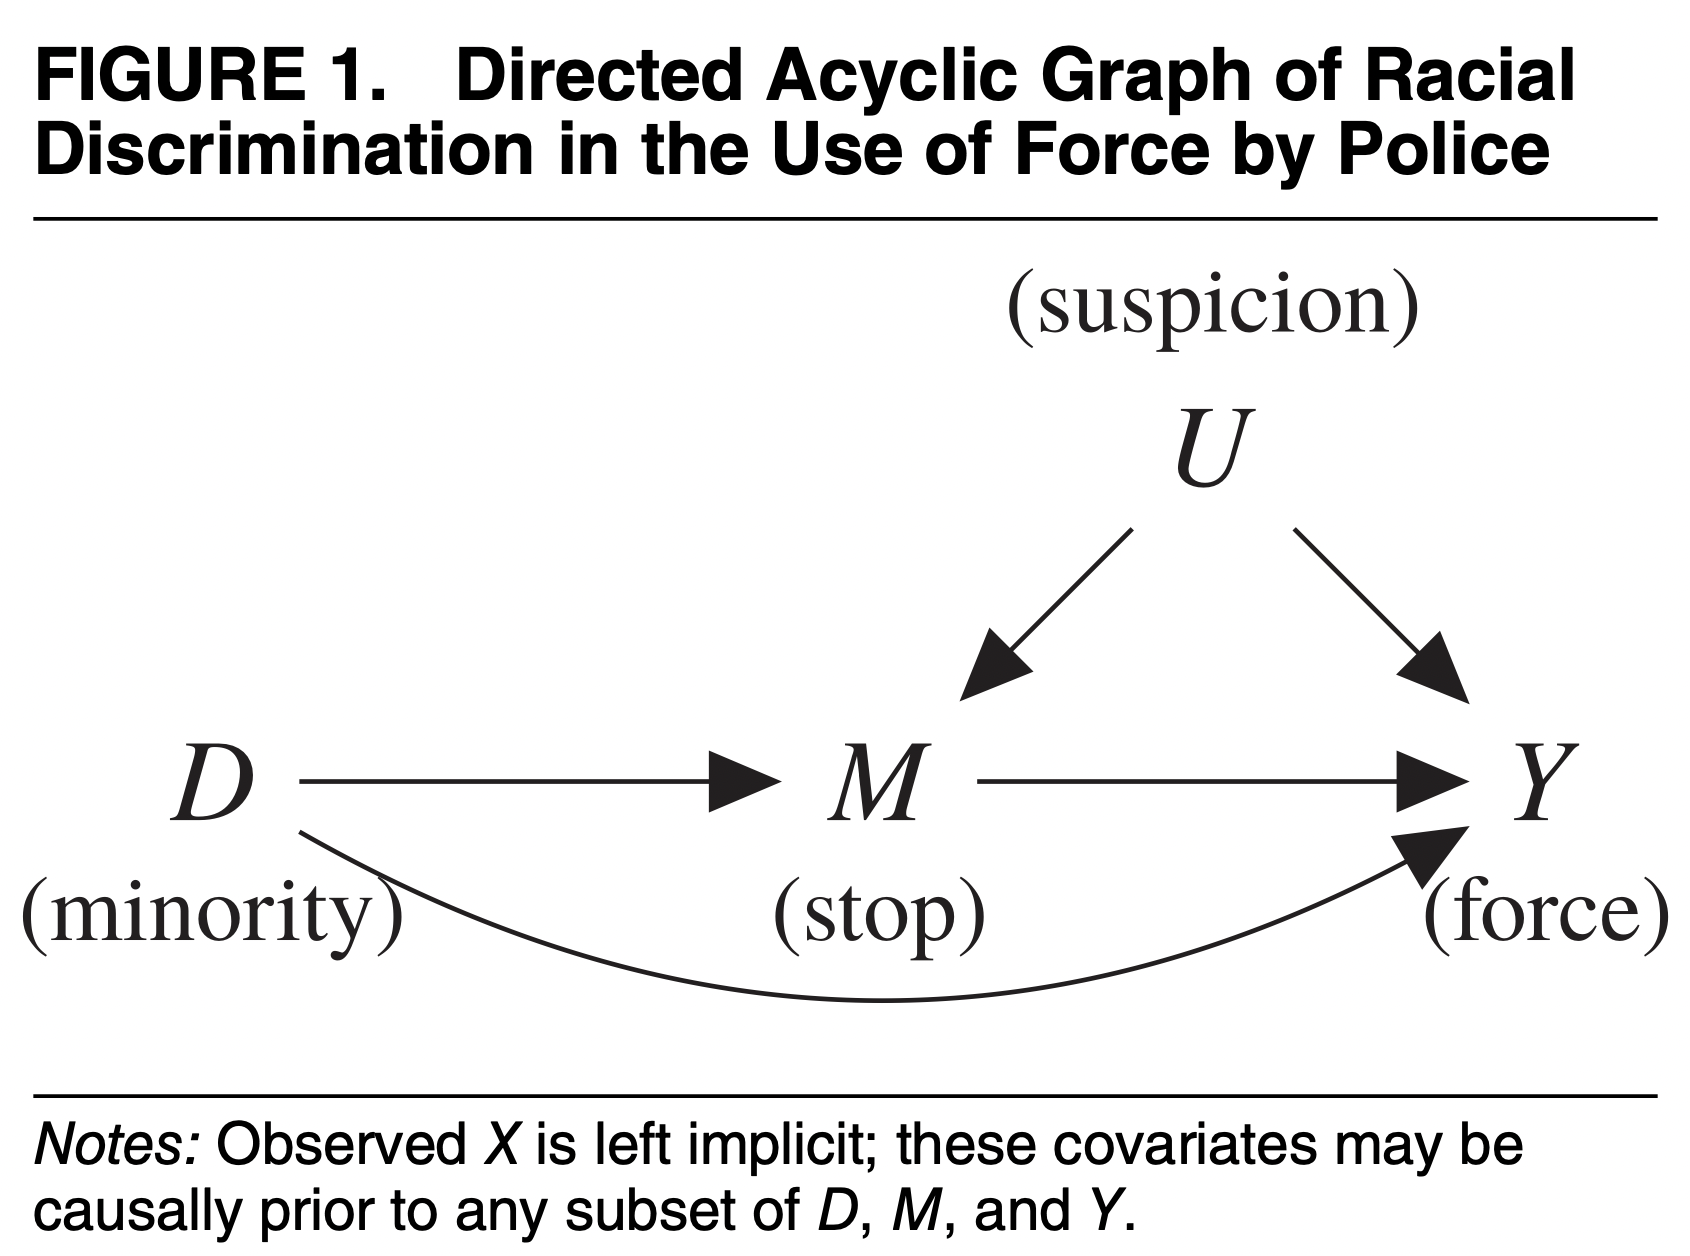
\includegraphics[height = .7\textheight]{figures/klm_fig1}
\end{frame}

\begin{frame}
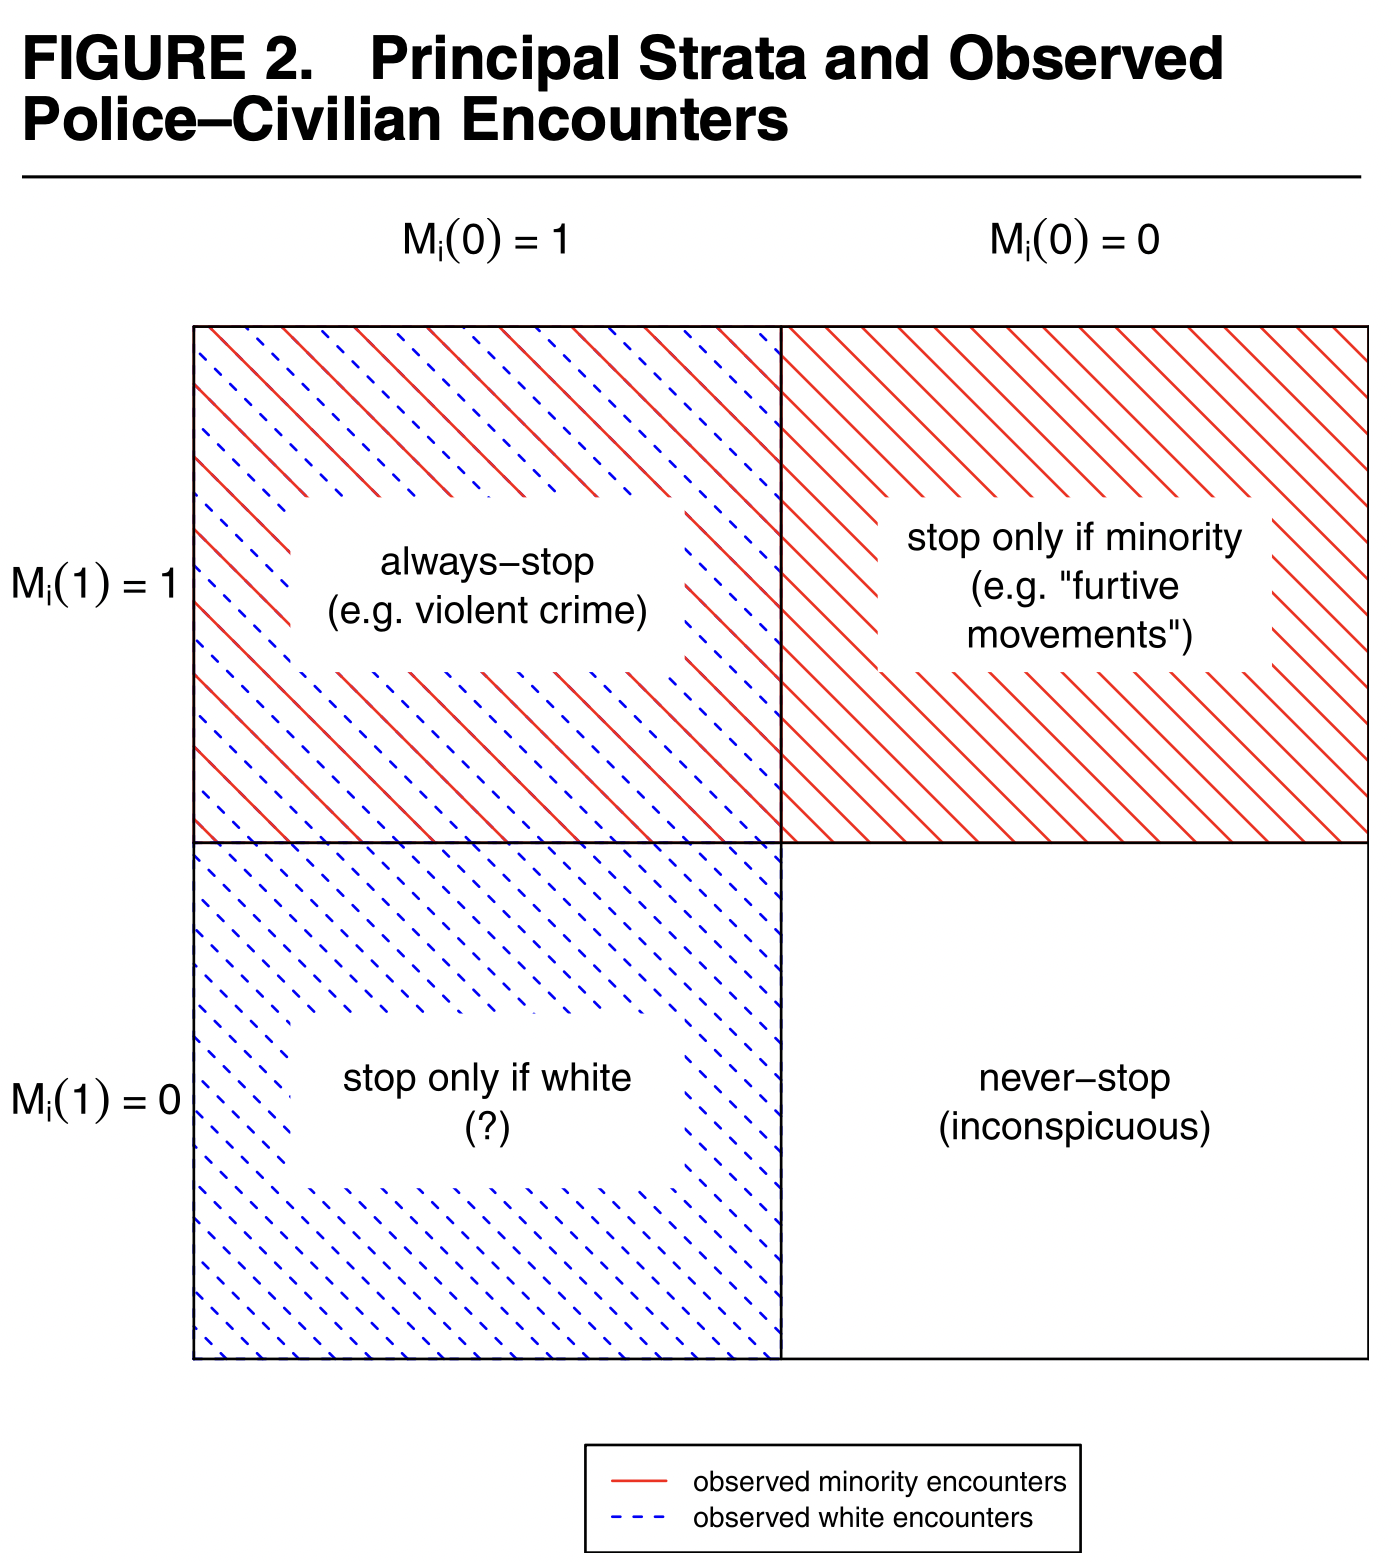
\includegraphics[height = .9\textheight]{figures/klm_fig2}
\end{frame}

\begin{frame}
We would want the ATE
$$\E(Y^{1M^1}-Y^{0M^0})$$ \vskip .2in
To estimate that, the authors say we need two things
\begin{enumerate}
\item Count of minority encounters\footnote{(including all four strata)}
\item Count of white encounters
\end{enumerate}
within strata of $X$
\end{frame}

\begin{frame}{Point estimates\hfill\begin{footnotesize}Note: All steps are within $X$. Notation dropped.\end{footnotesize}} \pause
\bgray{Important caveat:} \vskip .2in
The following is my reconstruction of one of the simplest of many results in Knox, Lowe, \& Mummolon 2020.
\end{frame}

\begin{frame}[t]{Point estimates\hfill\begin{footnotesize}Note: All steps are within $X$. Notation dropped.\end{footnotesize}}
\small
What proportion of encounters would involve\\force if they involved a minority civilian? \pause
$$\begin{aligned}
\E(Y^1) \pause
&= \E(Y^1\mid D = 1) &\text{Exchangeability} \\
\\ \pause
&= \E(Y\mid D = 1) &\text{Consistency} \\
\\ \pause
&= \overbrace{
		\P(M = 1\mid D = 1)
	}^{\onslide<6->{\substack{\text{Stop rate among}\\\text{minority encounters}}}}
	\overbrace{
		\E(Y\mid D = 1, M = 1)
	}^{\onslide<7->{\substack{\text{Use of force among}\\\text{stopped minority encounters}}}}
	  &\text{Law of Total}\\
&\qquad + \underbrace{
		\P(M = 0\mid D = 1)
	}_{\onslide<8->{\substack{\text{Non-stop rate among}\\\text{minority encounters}}}}
	\underbrace{
		\E(Y\mid D = 1, M = 0)
	}_{\onslide<9->{\substack{\text{Use of force among}\\\text{non-stopped minority encounters}\\(=0)}}}
	 &\text{Probability} \\
\\ 
\onslide<10->{
&= \overbrace{
		\P(M = 1\mid D = 1)
	}^{\substack{\text{Stop rate among}\\\text{minority encounters}}}
	\overbrace{
		\E(Y\mid D = 1, M = 1)
	}^{\substack{\text{Use of force among}\\\text{stopped minority encounters}}}
}
\end{aligned}$$
\end{frame}

\begin{frame}[t]{Point estimates\hfill\begin{footnotesize}Note: All steps are within $X$. Notation dropped.\end{footnotesize}}
\small
What proportion of encounters would involve\\force if they involved a minority civilian?
$$\begin{aligned}
\E(Y^1)
&= \overbrace{
		\P(M = 1\mid D = 1)
	}^{\substack{\text{Stop rate among}\\\text{minority encounters}}}
	\overbrace{
		\E(Y\mid D = 1, M = 1)
	}^{\substack{\text{Use of force among}\\\text{stopped minority encounters}}}
\end{aligned}$$ \pause
vs if they involved a non-minority civilian? \pause
$$\begin{aligned}
\E(Y^0)
&= \overbrace{
		\P(M = 1\mid D = 0)
	}^{\substack{\text{Stop rate among}\\\text{non-minority encounters}}}
	\overbrace{
		\E(Y\mid D = 0, M = 1)
	}^{\substack{\text{Use of force among}\\\text{stopped non-minority encounters}}}
\end{aligned}$$ \pause
Difference is the ATE. \vskip .1in \pause
You just needed to augment the data with stop rates! \pause \vskip .1in
Works because of two key factors: \pause
\begin{itemize}
\item Race is assumed exchangeable given $X$ \pause
\item When $M = 0$ (no stop), then $Y = 0$ (no force)
\end{itemize}
\end{frame}

\begin{frame}{Many possible estimands}
\begin{center}
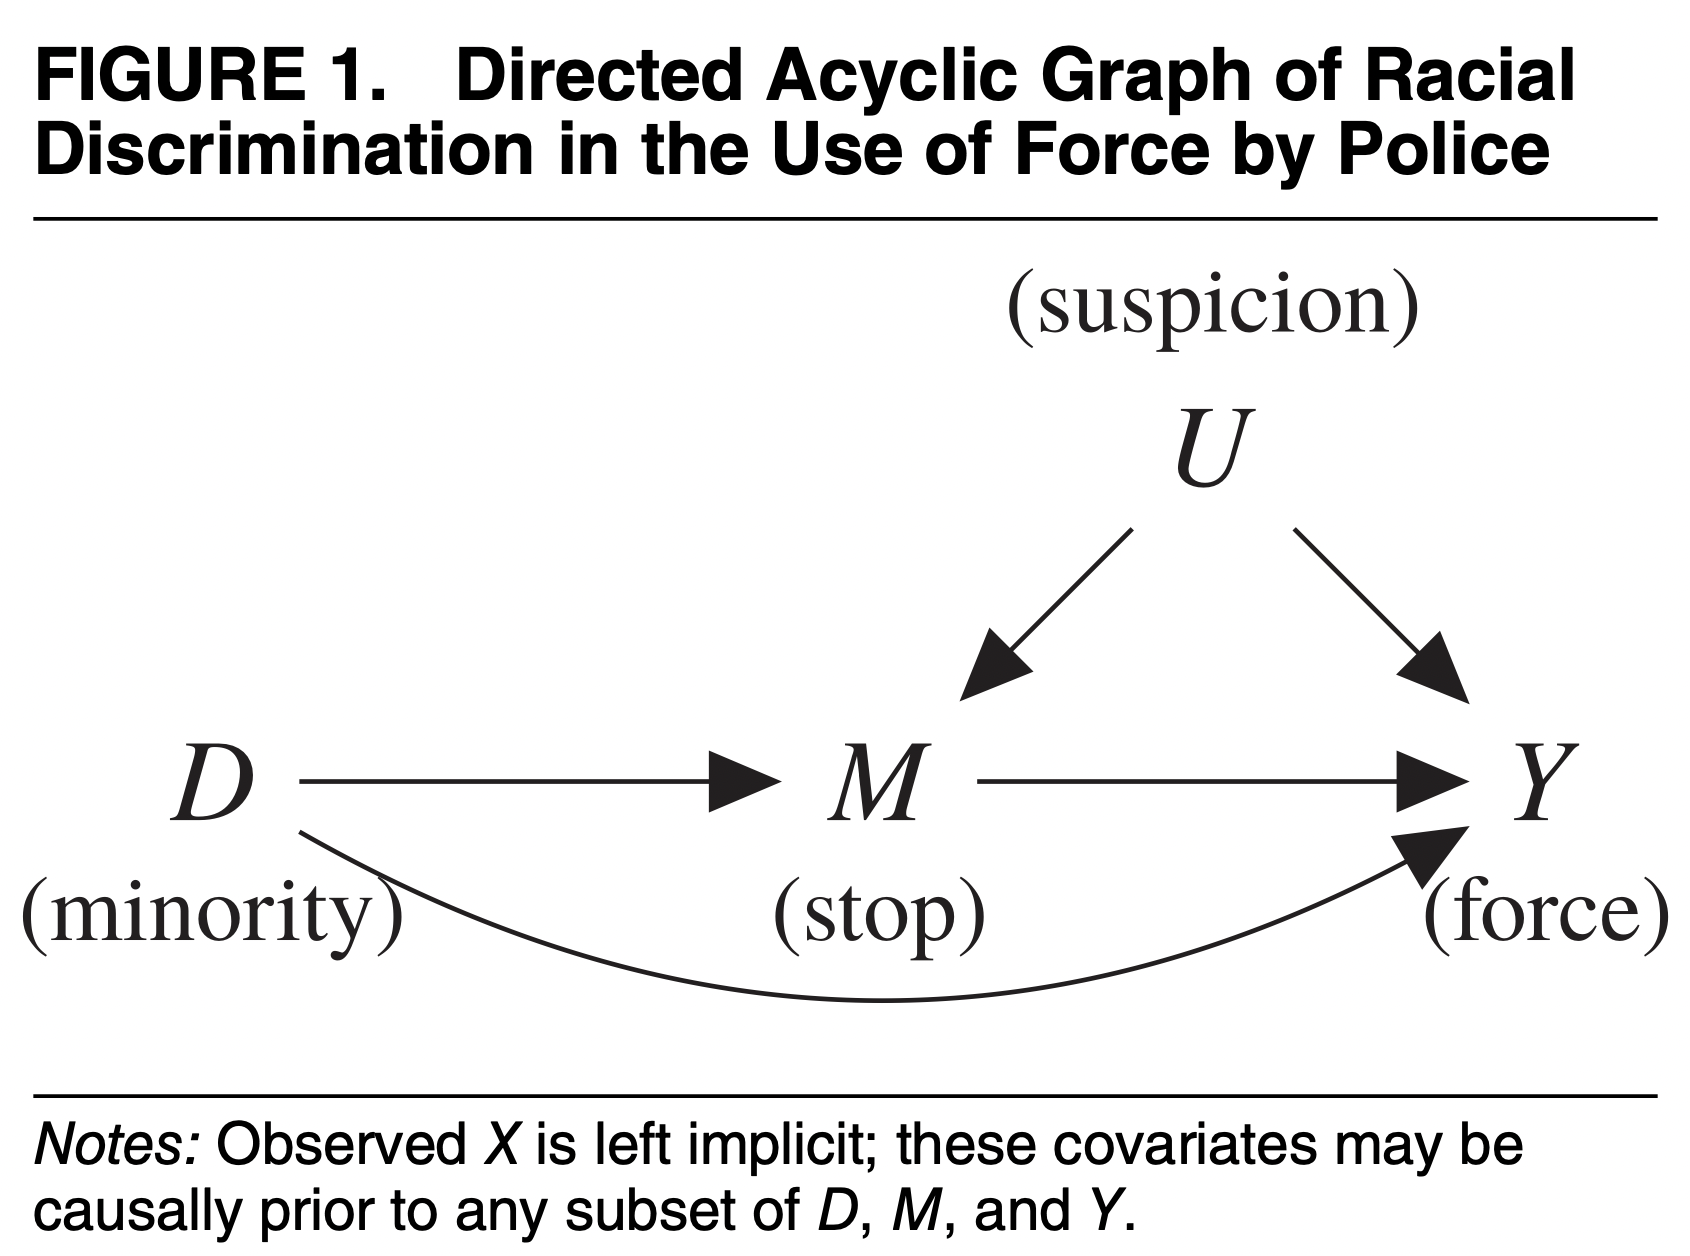
\includegraphics[height = .25\textheight]{figures/klm_fig1}
\end{center} \vskip .1in \pause
\begin{itemize}
\item ATE: $\E(Y^{1M^1} - Y^{0M^0})$
\begin{itemize} \pause
\item Racial bias, where non-stops are coded $Y = 0$ \pause
\end{itemize}
\item CDE: $\E(Y^{11} - Y^{01})$ \pause
\begin{itemize}
\item Racial bias if we stopped everyone \pause
\end{itemize}
\item ATE among the stopped \pause
\begin{itemize}
\item $\text{ATE}_{M = 1} = \E(Y^{1M^1} \mid M = 1) - \E(Y^{0M^0}\mid M = 1)$ \pause
\end{itemize}
\item Proportion of minority stops due to race \pause
\begin{itemize}
\item $\E(Y^{1M^1} - Y^{0M^0}\mid D = 1, M = 1)$
\end{itemize}
\end{itemize}
\end{frame}

\begin{frame}{Many estimands: Necessary Assumptions}

\begin{enumerate}
\item Mandatory reporting: $Y_i^{d0} = 0$ for all $i$ and $d$
\item Mediator monotonicity: $M_i^1\geq M_i^0$
\item Relative nonseverity of racial stops:
$$\begin{aligned}
&\E(Y^{dm}\mid D = d', \overbrace{M^1 = 1, M^0 = 1}^\text{Always Stop Stratum}, X) \\
&\geq \E(Y^{dm}\mid D = d',\underbrace{M^1 = 1, M^0 = 0}_\text{Racial Stop Stratum}, X)
\end{aligned}$$
\item Treatment ignorability
\begin{itemize}
\item $M^d\indep D\mid X$
\item $Y^{dm}\indep D\mid M^0, M^1, X$
\end{itemize}
\end{enumerate}

\end{frame}

\begin{frame}{Many Estimands: Necessary Assumptions}

Assume absence of $W$ and $V$. Ok to have $U$. \vskip .2in

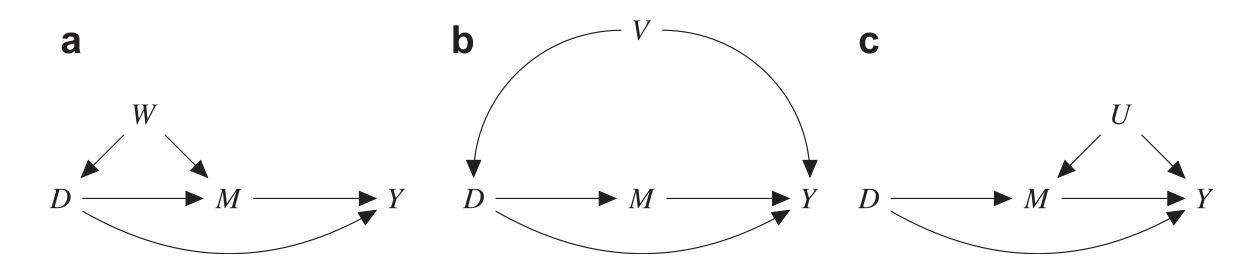
\includegraphics[width = \textwidth]{figures/klm_fig3}

\end{frame}


\begin{frame}{Many Estimands: Strong (As In Doubtful) Assumptions}

Studies about the effect of race conditional\\on an interaction implicitly assume these things:
\begin{enumerate}
\item Mediator ignorability: $Y^{dm}\indep M^0\mid D = d, M^1 = 1, X$
\begin{itemize}
%\item In encounters where an officer would stop a minority ($M^1 = 1$),\\whether that officer would stop a non-minority ($M^0$) is independent of whether they would use force if they stopped them ($Y^{dm}$)
\item ``violence rates in always-stop encounters must be identical to those in observationally equivalent racial stops''
\end{itemize}
\item No racial stops: $M^0 = M^1\mid M = 1$
\begin{itemize}
\item ``all reported encounters were of the always-stop kind''
\end{itemize}
\end{enumerate} \vskip .3in
Knox, Lowe, \& Mummolo argue that the above are implausible assumptions in the context of policing.

\end{frame}

\begin{frame}{Without the strong assumptions, things can be learned}
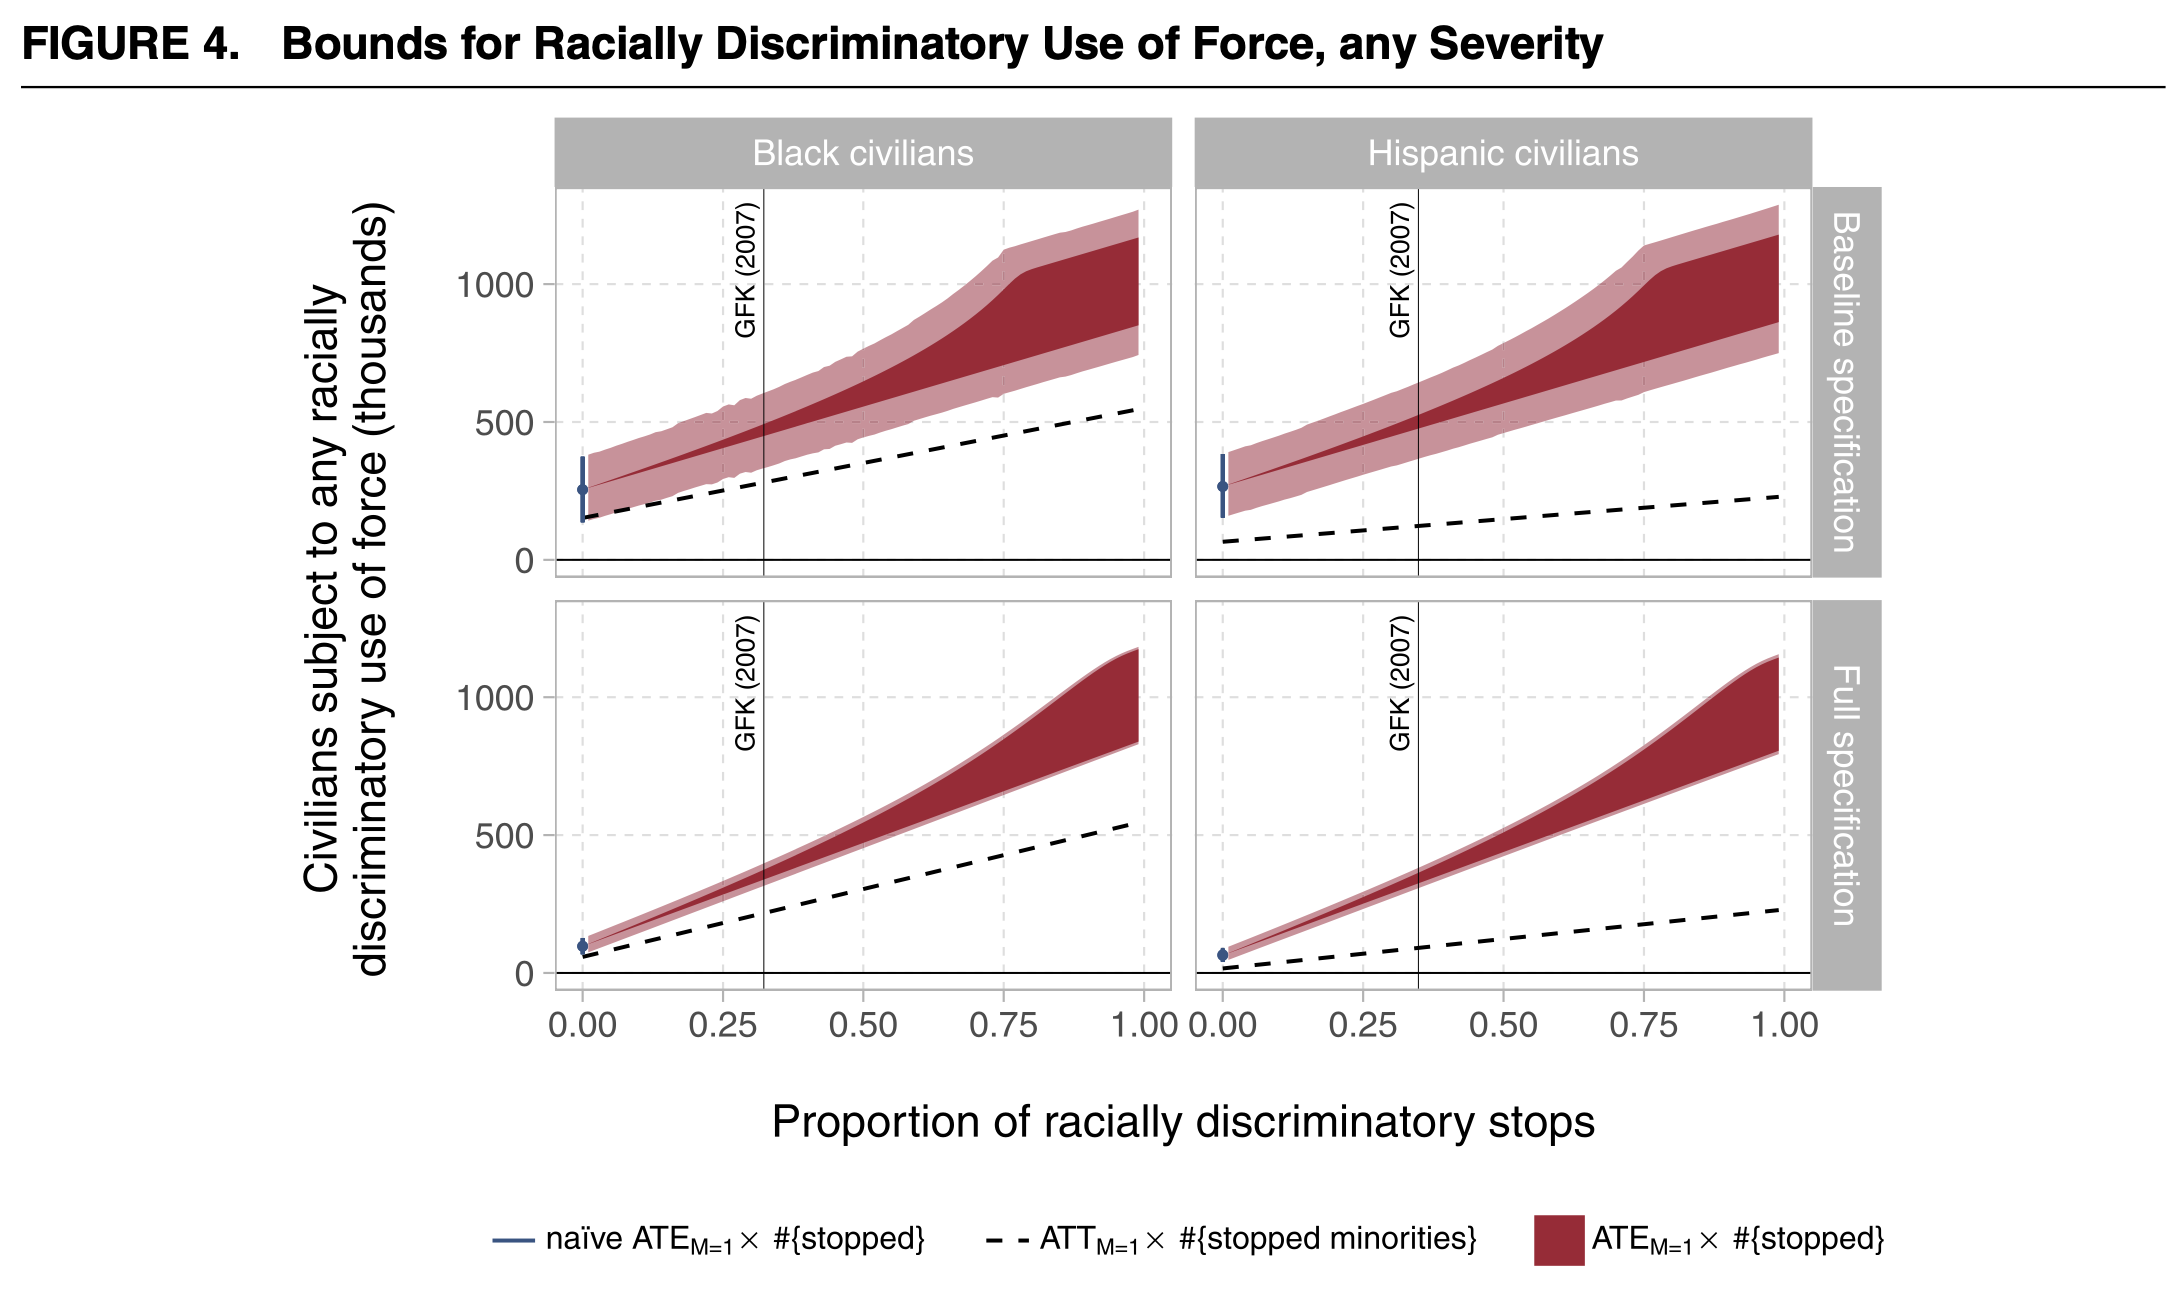
\includegraphics[height =.8\textheight]{figures/klm_fig4}
\end{frame}


\goalsframe


\begin{frame}{Let me know what you are thinking}

\begin{huge} \bref{https://tinyurl.com/CausalQuestions}{tinyurl.com/CausalQuestions} \end{huge}
\vskip .7in

Office hours TTh 11am-12pm and at \bref{https://calendly.com/ianlundberg/office-hours}{calendly.com/ianlundberg/office-hours}\\Come say hi!

\end{frame}


\end{document}
